% AGORA: Agent-based Government Open-data Reasoning Assistant
% ICWS 2026 — IEEE International Conference on Web Services
% Format: US Letter, two-column IEEE style. Double-blind: use anonymous block for submission.

\documentclass[conference,letterpaper]{IEEEtran}
\usepackage[utf8]{inputenc}
\usepackage[T1]{fontenc}
\usepackage{amsmath,amssymb}
\usepackage{graphicx}
\usepackage{booktabs}
\usepackage{hyperref}
\usepackage{xcolor}
\usepackage{balance}
\usepackage{url}

\hypersetup{colorlinks=true, linkcolor=blue, citecolor=blue, urlcolor=blue}

\title{AGORA: Agent-based Government Open-data Reasoning Assistant}

% Double-blind SUBMISSION: keep the line below (no names/affiliations).
\author{\IEEEauthorblockN{Anonymous Author(s)}}
% CAMERA-READY: comment out the line above and uncomment the block below.
%\author{
%\IEEEauthorblockN{Author Name(s)}
%\IEEEauthorblockA{Affiliation\\
%Email}
%}

\begin{document}

\maketitle

\begin{abstract}
We present AGORA (Agent-based Government Open-data Reasoning Assistant), an intelligent system that gives \emph{easy access} for any person to large government data portals. Data on such portals is often scarce, spread out, and hard to pinpoint without a background in data analytics; AGORA makes finding and retrieving information from open government data much simpler. Users ask natural-language questions (e.g., ``What is the feasibility of opening a restaurant in Paris?'' or ``Analyze the feasibility of building a hotel in Lyon'') and receive comprehensive, data-driven reports covering zoning, competition, demographics, and infrastructure. This aligns with the core goal of open government portals: to make data more accessible and to boost economic growth and contributions from citizens, organizations, and enterprises. AGORA is designed as a framework applicable to any open government data portal; we instantiate it over France's data.gouv.fr (~73k datasets). The pipeline orchestrates five specialized agents: a planner that decomposes questions into retrieval-oriented subqueries, hybrid (vector + BM25) search over dataset metadata, a dataset selector that assigns each hit to RAG or technical execution, a dual-path evidence layer (General agent with chunk retrieval vs.\ Technical agent with \textbf{Recursive Language Model (RLM)} for computation over structured data), and a synthesis agent that produces a single attributed answer. We describe challenges addressed---vector store and embedding design, dual-agent (GA/TA) design, RLM-based computation, broad resource-type support via the Unstructured library, query enrichment via a planner, on-demand resource download (no pre-storage of ~70k files), and relevance-based chunking---and discuss a systems-engineering perspective: agents as components in a ``factory,'' where adding more agents (e.g., description-quality filtering, synthesis validation) can further improve the pipeline. We report design findings and end-to-end usage/cost tracking; the system supports streaming and scales with self-hosted Weaviate and bring-your-own embeddings.
\end{abstract}

\begin{IEEEkeywords}
AGORA, open government data, question answering, multi-agent systems, RAG, hybrid search, recursive language model (RLM), DSPy, Weaviate, Unstructured, data.gouv.fr.
\end{IEEEkeywords}

%------------------------------------------------------------------------------
\section{Introduction}
\label{sec:intro}

Open government data portals expose large catalogues of datasets (tens of thousands) with heterogeneous formats---tabular (CSV, XLSX), record-based (JSON, GeoJSON), and documents (PDF, DOCX). Yet data is often scarce from a user's perspective, spread across many datasets, and hard to pinpoint without a background in data analytics. The very goal of these portals is to make data more accessible and to boost economic growth and contributions from citizens, organizations, and enterprises. AGORA addresses this gap by making \emph{finding and retrieving} information from open government data much simpler: any person can ask natural-language questions (e.g., ``What is the feasibility of opening a restaurant in Paris?'' or ``Analyze tourism data for Tours'') and receive actionable, data-driven answers. Enabling this poses several technical challenges: (1) mapping broad or multi-faceted questions to relevant datasets; (2) deciding whether to treat a dataset as context for summarization (RAG) or as structured data for computation; (3) combining evidence from multiple sources with clear attribution; and (4) controlling cost and latency in a pipeline that involves multiple large language model (LLM) and embedding calls.

We present \textbf{AGORA} (Agent-based Government Open-data Reasoning Assistant), an intelligent platform where AI agents autonomously collect and analyze open government data to answer such queries. Users interact through natural language (e.g., ``Analyze the feasibility of opening a restaurant in Lyon'' or ``What open data exists for Tours?'') and receive comprehensive reports covering zoning, competition, demographics, and infrastructure. AGORA is designed as a \emph{framework} applicable to any open government data portal; the current instantiation targets France's data.gouv.fr (~73k datasets). The system addresses these challenges through a fixed pipeline of specialized agents rather than a single RAG stack. The main contributions are:

\begin{itemize}
  \item An \textbf{orchestrator} that runs: planning $\rightarrow$ hybrid retrieval $\rightarrow$ dataset selection (with per-dataset execution mode) $\rightarrow$ evidence extraction (RAG or technical per dataset) $\rightarrow$ synthesis.
  \item A \textbf{dataset selector} that (1)~\emph{filters} the retrieval hits to only those datasets that are relevant or beneficial for the subquery---only some of the hits, or even none (e.g., when the French open government portal has no pertinent data for that subquery), may be relevant---and (2)~assigns each selected dataset to \emph{rag} (when a random sample of the resource suffices as context) or \emph{technical} (when the user question requires search or computation over the full data).
  \item A \textbf{dual-path evidence layer}: a General (RAG) agent using download $\rightarrow$ text extraction $\rightarrow$ chunking $\rightarrow$ embedding-based retrieval $\rightarrow$ LLM, and a Technical agent using structure detection $\rightarrow$ parsing into records $\rightarrow$ schema and preview $\rightarrow$ DSPy Recursive Language Model (RLM) with a sandboxed REPL, with fallback to unstructured extraction for non-tabular resources.
  \item \textbf{End-to-end usage and cost tracking} for LLM and embedding tokens across the pipeline, with optional cost estimates for known Azure OpenAI models.
  \item Design findings on query decomposition for hybrid search, on RAG vs.\ technical mode selection, and on decomposition, mode selection, attribution, and scalability; plus challenges addressed (Section~\ref{sec:challenges}) and a systems-engineering (``factory'') perspective on extensibility.
\end{itemize}

The rest of the paper is organized as follows. Section~\ref{sec:related} reviews related work. Section~\ref{sec:architecture} describes the architecture and orchestrator. Section~\ref{sec:challenges} summarizes the challenges addressed. Sections~\ref{sec:planner}--\ref{sec:synthesis} detail each agent and retrieval. Section~\ref{sec:implementation} covers implementation (DSPy, Weaviate, Unstructured, resource types). Section~\ref{sec:findings} discusses design findings and the factory perspective. Section~\ref{sec:conclusion} concludes.

%------------------------------------------------------------------------------
\section{Related Work}
\label{sec:related}

\textbf{RAG and open-domain QA.} Retrieval-augmented generation~\cite{lewis2020rag} grounds LLM answers in retrieved documents; recent surveys~\cite{gao2023rag, huang2024rag} summarize the field. Most work focuses on document-level retrieval and single-step generation. AGORA instead operates over \emph{dataset metadata} for discovery, then fetches and processes \emph{resources} (files) per selected dataset, and supports both passage-style context (RAG) and structured, computation-oriented analysis (technical path).

\textbf{Query decomposition and multi-step retrieval.} Decomposing complex questions into subqueries improves retrieval coverage~\cite{xiong2021multihop, wolfson2020break, fu2021decomposing}; decomposition for RAG is explicitly studied in recent work~\cite{ammann2025decomposition}. AGORA's planner produces subqueries explicitly designed for hybrid dataset search (vector + BM25) and optionally breaks broad questions into multiple retrieval themes (e.g., tourism, infrastructure) to improve recall across domains.

\textbf{Hybrid search.} Combining dense (vector) and sparse (e.g., BM25) retrieval is standard in modern search stacks~\cite{lee2023hybrid, wang2024rag}. AGORA uses Weaviate's hybrid search with a configurable $\alpha$ (default 0.5) over dataset title, description, and organization, with vectors from a bring-your-own embedding model (e.g., Azure OpenAI \texttt{text-embedding-3-small}).

\textbf{Language models and code execution.} Recursive (or agentic) language models that can execute code in a sandbox enable precise computation over tables and JSON~\cite{gao2023pal, chen2022program, cheng2023binder, wang2024chainoftable, zhang2024reactable}; the RLM paradigm is formalized in recent work~\cite{zhang2025rlm}. AGORA's Technical agent uses DSPy's RLM with a sandboxed Python REPL to explore schema and preview data and to produce structured evidence---\emph{introducing RLM for government open data analysis}---falling back to a single Predict call when the REPL is unavailable.

\textbf{Open government data and data portals.} Data portals typically expose catalogues via APIs; discovery and reuse remain difficult for non-experts~\cite{nikiforova2021usability, molodtsov2024usability}, yet the mission of open government is to make data accessible and to foster economic growth and contributions from citizens, organizations, and enterprises~\cite{wang2023ogd}. AGORA is designed as a framework for any such portal, simplifying finding and retrieving information so that any person can benefit without data analytics expertise; we instantiate it over data.gouv.fr's public API, embedding dataset metadata for semantic and keyword search and bridging from metadata to on-demand file download and content extraction.

%------------------------------------------------------------------------------
\section{Architecture and Orchestrator}
\label{sec:architecture}

The pipeline is linear and deterministic per question: no loops or dynamic tool choice beyond the selector's per-dataset mode; it fits the multi-agent workflow view of specialized components (planner, retriever, selector, executor, synthesis) discussed in recent surveys~\cite{li2024multiagent}. Figure~\ref{fig:pipeline} summarizes the flow.

\begin{figure}[t]
  \centering
  \fbox{\parbox{0.92\columnwidth}{
    \small
    \textbf{1. Planner} $\rightarrow$ intent + subqueries \\
    \textbf{2. For each subquery:} \\
    \quad 2a. \textbf{Retrieval}: hybrid search $\rightarrow$ top-$k$ dataset hits \\
    \quad 2b. \textbf{Dataset selector}: filter + assign \texttt{rag} or \texttt{technical} per hit \\
    \quad 2c. \textbf{Per selected dataset}: General (RAG) or Technical agent $\rightarrow$ evidence block \\
    \textbf{3. Synthesis}: concatenated evidence + plan context $\rightarrow$ final answer \\
    \textbf{4. Response}: answer, plan, evidence, hits, usage/cost
  }}
  \caption{High-level pipeline.}
  \label{fig:pipeline}
\end{figure}

Figure~\ref{fig:sequence} gives a simplified sequence: the orchestrator calls the planner once, then for each subquery runs retrieval $\rightarrow$ selector $\rightarrow$ (General or Technical) per selected dataset; evidence is concatenated and passed to synthesis. The design mirrors a production line: each agent has a well-defined input/output; adding more agents (e.g., a step to filter low-quality dataset descriptions before embedding, or to validate synthesis output) can be done without changing the core flow.

\begin{figure}[t]
  \centering
  \fbox{\parbox{0.92\columnwidth}{
    \small
    \textbf{Sequence:} User $\rightarrow$ Orchestrator $\rightarrow$ Planner (intent + subqueries). \\
    For each subquery: search\_datasets (Weaviate hybrid) $\rightarrow$ Selector (selected\_datasets + mode) $\rightarrow$ for each selected: GeneralAgent or TechnicalAgent $\rightarrow$ evidence. \\
    Orchestrator concatenates evidence $\rightarrow$ SynthesisAgent $\rightarrow$ answer $\rightarrow$ User.
  }}
  \caption{Simplified call sequence (orchestrator-centric).}
  \label{fig:sequence}
\end{figure}

\subsection{Orchestrator}

The \textbf{AgentOrchestrator} (orchestrator) is the single entry point. It holds references to: PlannerAgent, GeneralAgent, TechnicalAgent, DatasetSelectorAgent, and SynthesisAgent. It does not call the retrieval or embedding clients directly; retrieval is invoked via a pipeline helper that returns hits and embedding usage for cost tracking.

Two execution modes are supported at runtime:
\begin{itemize}
  \item \textbf{General-only (RAG-only):} A global flag (\texttt{USE\_ONLY\_GENERAL\_AGENT}) forces every selected dataset to be executed with the General agent. The selector may still choose which datasets to keep, but execution mode is overridden to \texttt{rag}.
  \item \textbf{Technical mode:} The selector's output is respected: each selected dataset is run with either the General agent or the Technical agent according to \texttt{execution\_mode}.
\end{itemize}

The orchestrator supports both a blocking \texttt{run(question, k)} and a streaming variant that yields server-sent events (SSE): \texttt{status}, \texttt{plan}, \texttt{user\_message}, \texttt{error}, and \texttt{done} with the full response. This allows the front-end to show progress (e.g., ``Searching datasets for: …'', ``Checking dataset: …'') and the final answer without waiting for the entire pipeline.

\subsection{Data flow}

\begin{itemize}
  \item \textbf{Input:} User question (string), $k$ (number of retrieval hits per subquery).
  \item \textbf{Plan:} Intent (string) and a list of subqueries, each with \texttt{question} and \texttt{purpose}.
  \item \textbf{Hits:} Per subquery, hybrid search returns a list of dataset objects (dataset\_id, title, description, organization, url, tags, scores). Hits are deduplicated by \texttt{dataset\_id} per subquery.
  \item \textbf{Selection:} For each subquery, the selector returns a list of \texttt{SelectedDataset(dataset\_id, execution\_mode, reasoning)}. Only these datasets are executed; others are skipped.
  \item \textbf{Evidence:} Each executed dataset produces an \texttt{ExecutionResult(mode, subquery, evidence, lm\_usage, embed\_usage)}. Evidence is free-form text (RAG summary or technical analysis).
  \item \textbf{Synthesis:} All evidence strings are concatenated (with implicit ordering by subquery and dataset). The synthesis agent also receives the plan intent, subquery lines, and dataset references (title, organization, URL) so it can cite sources and include links in the final answer.
  \item \textbf{Output:} \texttt{AgentResponse(answer, plan, evidence, hits, user\_messages, lm\_usage\_grand\_total, embed\_usage\_grand\_total)}.
\end{itemize}

\subsection{System interface and user experience}

Users interact with AGORA through a web front-end that connects to the streaming API. Before submitting a question, the user selects the \textbf{execution mode}: \textbf{General} (RAG-only for all selected datasets) or \textbf{Technical} (the dataset selector assigns each hit to RAG or technical execution). This choice makes the two-path design visible and allows non-experts to request either descriptive answers or computation-oriented analysis. During a run, the interface displays \textbf{real-time progress} via server-sent events. As shown in Figure~\ref{fig:progress}, each progress message includes the dataset currently being analyzed, the selected mode (RAG or Technical), an explanation for why the dataset is relevant (and potentially why that mode was chosen), and a user-friendly link to the dataset on the French open government data website (data.gouv.fr). Users can thus see exactly where their information comes from for every dataset used in the query. When the pipeline completes, the user sees the \textbf{synthesized answer} with attributed sources and dataset links. The synthesis agent is instructed to always include proper citations for any information provided, including URLs; Figure~\ref{fig:sample-output} shows a section of the output illustrating this. All agents are instructed to respond only from the provided dataset content and not to hallucinate, so that answers are always \textbf{data-driven} and honest. Figures~\ref{fig:interface-modes}--\ref{fig:sample-output} illustrate the interface: mode selection and query input, progress messages during a run, and a sample output.

\begin{figure}[t]
  \centering
  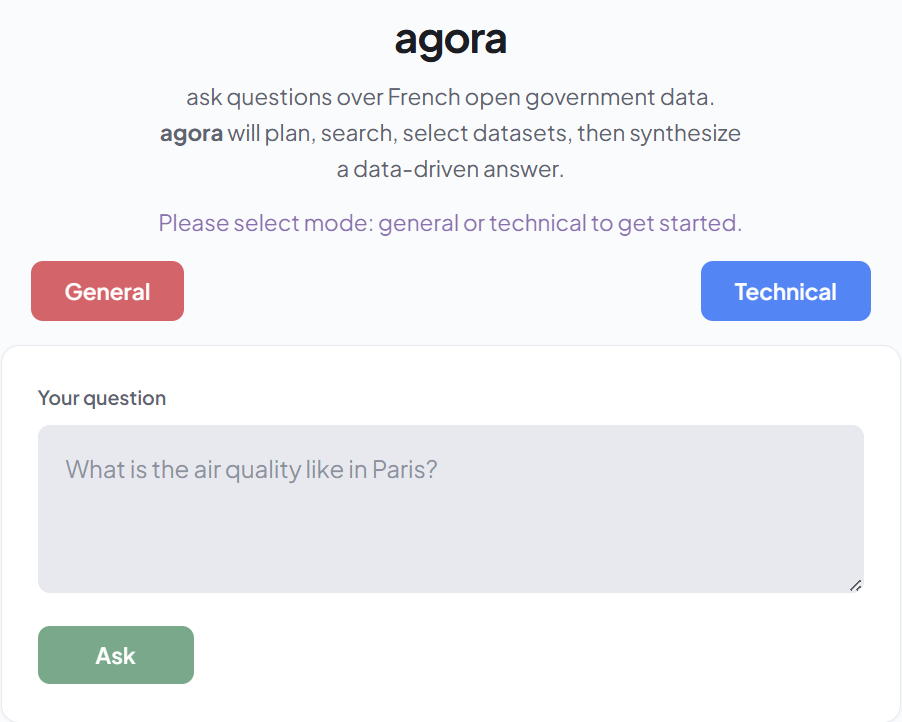
\includegraphics[width=\columnwidth]{fig_interface_modes}
  \caption{AGORA interface: choice between General (RAG-only) and Technical (RAG or technical per dataset) execution mode, and the natural-language query input.}
  \label{fig:interface-modes}
\end{figure}

\begin{figure}[t]
  \centering
  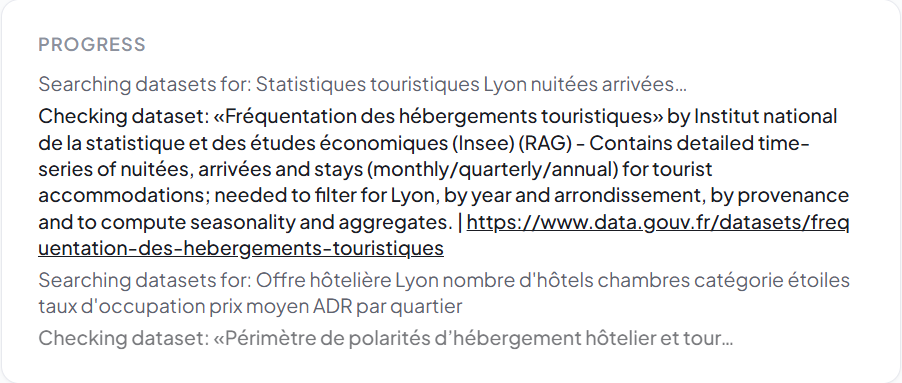
\includegraphics[width=\columnwidth]{fig_progress}
  \caption{Real-time progress: each message shows the dataset being analyzed, the selected mode (RAG or Technical), the selector's reasoning for relevance and mode, and a clickable link to the dataset on data.gouv.fr.}
  \label{fig:progress}
\end{figure}

\begin{figure}[t]
  \centering
  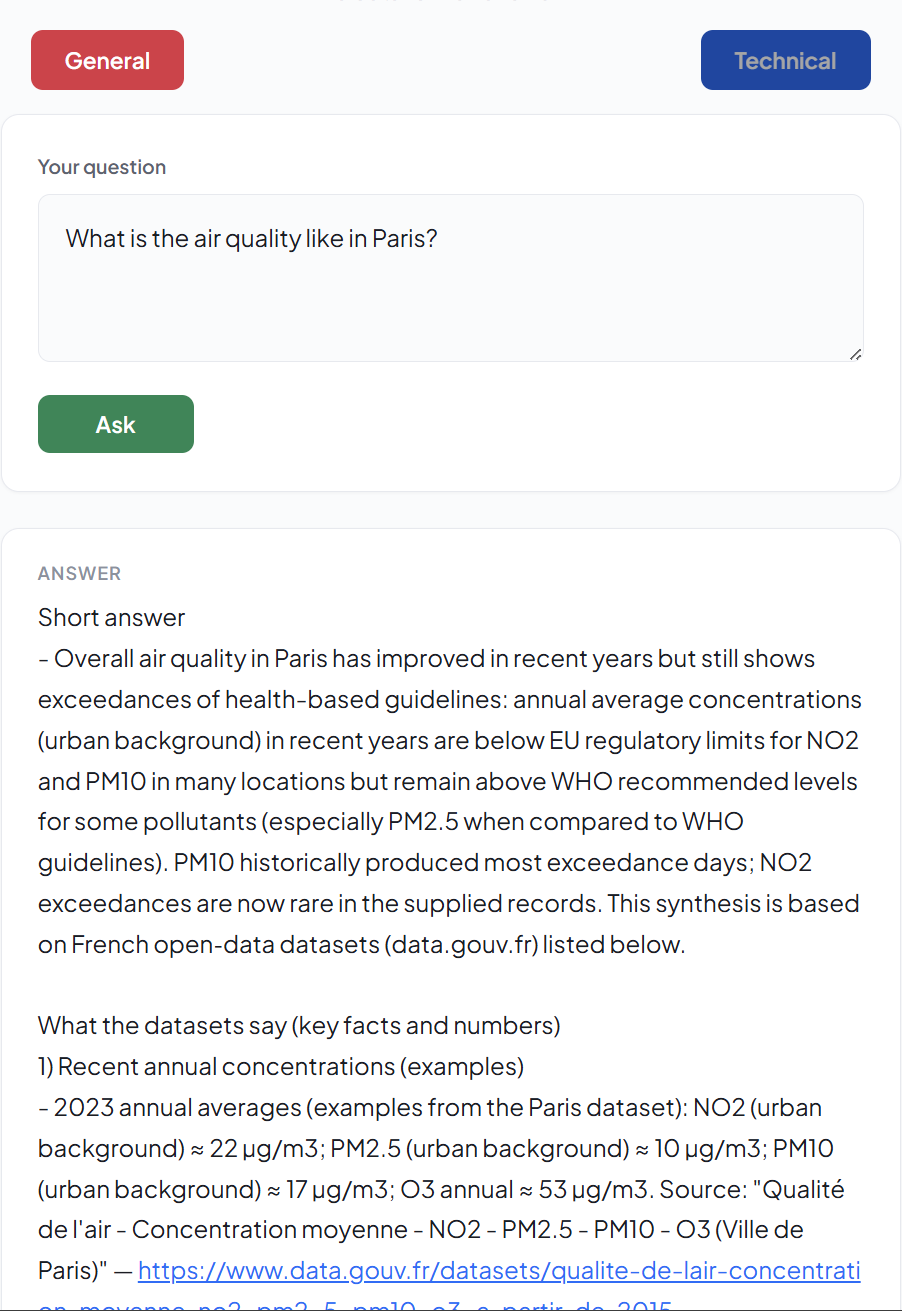
\includegraphics[width=\columnwidth]{fig_sample_output}
  \caption{Sample output (excerpt): the synthesis agent is instructed to include proper citations and URLs for all information; answers are grounded only in the provided datasets.}
  \label{fig:sample-output}
\end{figure}

Usage and cost are aggregated: the orchestrator merges LLM usage from planner, selector, each General/Technical call, and synthesis, and merges embedding usage from retrieval and from the General agent's chunk-retrieval step. When the configured models have known pricing (e.g., \texttt{gpt-5-mini}, \texttt{text-embedding-3-small}), the backend logs an estimated cost in USD for the run.

%------------------------------------------------------------------------------
\section{Challenges Addressed}
\label{sec:challenges}

During development we identified and solved the following challenges, which we summarize here for reproducibility and to guide similar systems.

\textbf{Vector store and hybrid search.} Storing and querying dataset metadata at scale (e.g., ~73k datasets) required a vector database. We use Weaviate (self-hosted) with \emph{self-provided} vectors: an external embedding client (Azure OpenAI) computes vectors at ingestion and at query time. Hybrid search (vector + BM25) with a configurable $\alpha$ improves recall over keyword-only or vector-only retrieval.

\textbf{Rich embeddings for dataset metadata.} To improve retrieval quality, the embeddable text for each dataset uses \emph{all} of: title, description, tags, and organization name. The ingestion pipeline builds a single \texttt{to\_embedding\_text()} string from these fields (with description truncation by token count to stay within model limits) so that both semantic and organizational context are available to the vector index.

\textbf{Two agents for different query types.} Not all questions are best answered by the same strategy. We introduced a \textbf{General Agent (GA)} for descriptive or overview-style questions (RAG: sample context, chunk, retrieve relevant chunks, generate answer) and a \textbf{Technical Agent (TA)} for computation-oriented questions (parse structured data, build schema + preview, use RLM to explore and compute). The dataset selector assigns each hit to GA or TA per dataset.

\textbf{Technical agent computation.} Enabling the TA to \emph{generate and perform} computation over government data is a key contribution. We use DSPy's \textbf{Recursive Language Model (RLM)}: the model writes and runs code in a sandboxed Python REPL to inspect, filter, and aggregate data, then submits a structured evidence block. This paper introduces the use of RLM for analyzing open government data in this way.

\textbf{Support for many resource types.} Open data portals expose heterogeneous formats. We support tabular (CSV, TSV, XLS, XLSX), record-based (JSON, JSONL, GeoJSON), documents (PDF, DOCX, HTML, XML, MD, PPT, PPTX, ODT, EPUB, RTF, RST), GTFS/GTFS-RT (ZIP with schedule files), and binary (e.g., protobuf) where extractable. The \textbf{Unstructured} library\footnote{\url{https://unstructured.io/}} is used for document and spreadsheet extraction (DOCX, XLSX, HTML, XML, etc.); PDF uses pypdf for stability; CSV/JSON/GeoJSON use pandas/json with size and row limits. Unsupported or oversized files yield a short fallback message rather than failing the pipeline.

\textbf{Query enrichment (Planner).} Adding context between ``user question'' and ``retrieve datasets'' improves relevance. The Planner agent decomposes the question into intent and one or more retrieval-oriented subqueries (e.g., ``feasibility of hotel in Lyon'' $\rightarrow$ tourism, infrastructure, roads). Each subquery is run against the vector store separately; the union of hits (deduplicated) increases coverage.

\textbf{On-demand resource download.} Pre-storing files for ~70k datasets would be expensive and redundant. Resources are \emph{downloaded as-needed} per user query: only datasets selected by the selector are fetched, and only up to a cap of resources per dataset. This keeps storage and ingestion cost low while still allowing full content access for the chosen datasets.

\textbf{Chunking and relevance-based context.} Feeding the entire extracted content to the LLM would exceed context limits and dilute relevance. In the General agent we \emph{chunk} extracted text (with size and overlap limits), embed chunks and the subquery, and select the top-$k$ chunks by cosine similarity---so that only parts relevant to the user question (e.g., containing ``Paris'' or related content) are passed to the model. A per-resource cap prevents a single large resource from dominating the context.

%------------------------------------------------------------------------------
\section{Planner Agent}
\label{sec:planner}

The \textbf{PlannerAgent} turns the user question into a \textbf{QueryPlan}: an intent (short summary of what the user wants) and one or more \textbf{SubQuery} items, each with a \texttt{question} (retrieval-oriented) and a \texttt{purpose} (why this subquery is needed).

Design rules encoded in the planner signature:
\begin{itemize}
  \item If the question is \emph{broad} and may span multiple dataset domains, decompose into several focused subqueries (e.g., ``feasibility of building a hotel in Lyon'' $\rightarrow$ tourism, infrastructure, roads).
  \item If the question is \emph{narrow} or specific enough, return a single subquery (the original or a slight reformulation optimized for hybrid dataset search).
  \item Subqueries must be concise and retrieval-ready (aligned with data discovery, not generic reasoning).
\end{itemize}

Implementation: DSPy \texttt{ChainOfThought(PlanSignature)}. The signature takes \texttt{question} and \texttt{current\_timestamp} (UTC ISO-8601) and outputs \texttt{output\_json} with \texttt{intent} and \texttt{subqueries}. The orchestrator parses this JSON and builds a \texttt{QueryPlan}; on parse failure it returns a minimal plan (intent = question, subqueries = []). LLM usage from the planner is recorded and merged into the pipeline grand total. Figure~\ref{fig:subqueries} shows example DSPy output from the planner for the user question ``What is the feasibility of building a hotel in Lyon?'': the generated intent and subqueries used for dataset retrieval.

\begin{figure}[t]
  \centering
  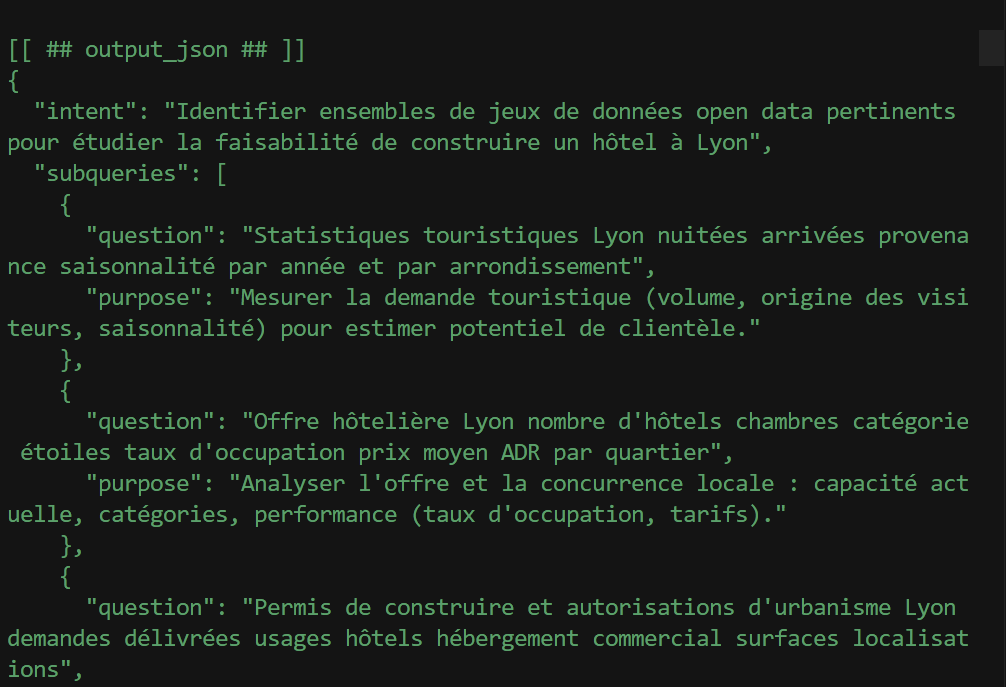
\includegraphics[width=\columnwidth]{subqueries_generated}
  \caption{Planner output (DSPy): intent and subqueries generated for the user question ``What is the feasibility of building a hotel in Lyon?'' used to drive hybrid search over the dataset index.}
  \label{fig:subqueries}
\end{figure}

%------------------------------------------------------------------------------
\section{Retrieval}
\label{sec:retrieval}

Dataset discovery uses \textbf{hybrid search} over a Weaviate collection. The collection stores: \texttt{dataset\_id}, \texttt{title}, \texttt{description}, \texttt{organization}, \texttt{content} (the text used for embedding and keyword match), \texttt{url}, \texttt{tags}. Vectors are \emph{self-provided}: ingestion uses an external embedding client (Azure OpenAI) to compute vectors and upsert (content, vector) along with metadata. At query time, the pipeline embeds the query text once per subquery, then calls Weaviate's \texttt{hybrid} search with \texttt{query\_text}, \texttt{query\_vector}, \texttt{k}, and \texttt{alpha}. The parameter $\alpha \in [0,1]$ balances vector similarity ($\alpha=1$) and keyword (BM25) score ($\alpha=0$); default is $0.5$.

Retrieval returns a list of hits (properties plus \texttt{\_distance}, \texttt{\_score}). Embedding usage for the query is returned to the orchestrator for pipeline-level embedding cost. No LLM is used in retrieval. Deduplication by \texttt{dataset\_id} is applied per subquery so that each dataset appears at most once per subquery.

%------------------------------------------------------------------------------
\section{Dataset Selector Agent}
\label{sec:selector}

The \textbf{DatasetSelectorAgent} has two main roles. First, it \emph{filters} the retrieval hits: hybrid search returns a top-$k$ list of candidate datasets, but only some---or even none---may actually be relevant to the subquery (e.g., the French open government portal may contain no datasets that address that particular theme). The selector keeps only those hits that are useful or beneficial for answering the question. Second, for each retained dataset it \emph{assigns} an execution mode (rag or technical). It receives the user question, the current subquery, and the list of retrieved hits (each with dataset\_id, title, description, organization) and outputs a list of \textbf{SelectedDataset} entries, each with:
\begin{itemize}
  \item \texttt{dataset\_id};
  \item \texttt{execution\_mode}: \texttt{rag} or \texttt{technical};
  \item \texttt{reasoning}: short explanation for why this dataset and this mode.
\end{itemize}

The selector may return an \emph{empty} list when none of the hits are relevant (off-topic, too generic, or simply absent from the portal for that subquery). This filtering step reduces unnecessary downloads and LLM calls.

Execution-mode semantics (exposed to the LLM in the signature):
\begin{itemize}
  \item \textbf{rag:} Use when a \emph{random sample} of the dataset resource is sufficient context (e.g., general description, overview, synthesis). The General agent will download resources, extract text, chunk, retrieve top-$k$ chunks by similarity, and ask the LLM to answer from that context.
  \item \textbf{technical:} Use when the question requires \emph{searching for something specific} (e.g., a particular record or value) or \emph{computing} over the data (e.g., largest value, mean, count, filter). The Technical agent will parse structured resources and use schema + preview + RLM (or Predict fallback).
\end{itemize}

Implementation: DSPy \texttt{ChainOfThought(DatasetSelectorSignature)}. Descriptions are truncated to a fixed character limit to avoid oversized prompts. The agent returns \texttt{output\_json}; the selector parses and validates the structure (e.g., \texttt{selected\_datasets} must be a list; \texttt{execution\_mode} must be \texttt{rag} or \texttt{technical}, defaulting to \texttt{rag}). Up to three attempts are made on parse/validation failure. Selected \texttt{dataset\_id}s that do not appear in the candidate hits are logged and skipped at execution time.

%------------------------------------------------------------------------------
\section{General (RAG) Agent}
\label{sec:general}

The \textbf{GeneralAgent} implements the RAG path: for each selected dataset (up to a cap, e.g., 3), it fetches the dataset from the data.gouv API, collects resource URLs, and for each resource (up to a cap, e.g., 5) downloads the file and extracts text. Extracted content is organized into \emph{evidence blocks} (resource\_id, metadata, content). Metadata is a short line (dataset title, organization, format, description, URL) for source attribution.

Optionally, \textbf{chunk retrieval} is enabled~\cite{yepes2024chunking, qu2024semantic, chen2024dense}: blocks are split into chunks (max size and overlap in characters), each chunk is embedded, and the subquery is embedded; cosine similarity ranks chunks. The top-$k$ chunks are selected with a \emph{per-resource cap} so that a single large resource does not dominate the context. If chunk retrieval is disabled or embedding fails, the full evidence text is used as context. The context is then truncated if a global character limit is set.

A single DSPy \texttt{Predict(AnswerFromContext)} call produces the evidence string: the LLM is prompted to answer the subquery using only the provided context, in the same language as the question, and to produce a self-contained block that the synthesis step can merge. The agent returns \texttt{ExecutionResult(mode=rag, subquery, evidence, lm\_usage, embed\_usage)}. Embedding usage from chunk retrieval (when used) is reported so the orchestrator can sum pipeline embedding cost.

%------------------------------------------------------------------------------
\section{Technical Agent}
\label{sec:technical}

The \textbf{TechnicalAgent} targets computation-oriented subqueries. For each selected dataset (up to a cap), it downloads resources and classifies each file:
\begin{itemize}
  \item \textbf{Tabular:} CSV, TSV, XLS, XLSX $\rightarrow$ parsed into records (with row/column limits and size guards to avoid OOM).
  \item \textbf{Records:} JSON (array of objects), JSONL, GeoJSON (FeatureCollection) $\rightarrow$ parsed into records.
  \item \textbf{Unsuitable:} Other formats (e.g., PDF) $\rightarrow$ same text extraction as the General agent; the extracted text is appended to an ``unstructured'' section of the technical context so the RLM can still use it.
\end{itemize}

A \textbf{technical context} string is built from: schema summaries (column names and types), preview rows (e.g., first 50 records per resource) as JSON, and optional unstructured blocks. This context is capped in length to avoid token overflow. The Technical agent then calls DSPy's \textbf{RLM} (Recursive Language Model) with a signature \texttt{ExploreTechnicalContext}: the model can run code in a sandboxed Python REPL to inspect, filter, and aggregate the data, and use \texttt{llm\_query} for semantic extraction, then \texttt{SUBMIT(answer)}. Limits (max iterations, max LLM calls) prevent runaway loops. If the RLM/REPL is unavailable (e.g., REPL not installed), the agent falls back to a single \texttt{Predict(ExploreTechnicalContext)} call with the same context. Figure~\ref{fig:rlm-code} shows an excerpt of Python code generated and executed by the RLM during technical mode.

\begin{figure}[t]
  \centering
  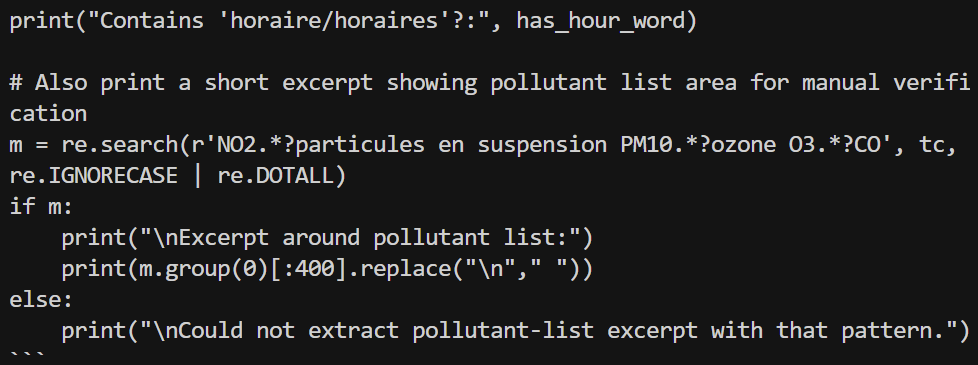
\includegraphics[width=\columnwidth]{python_code_excerpt}
  \caption{Excerpt of Python code generated and run by the RLM (Technical agent) in the sandboxed REPL during technical-mode analysis of a dataset.}
  \label{fig:rlm-code}
\end{figure}

The result is returned as \texttt{ExecutionResult(mode=technical, subquery, evidence, lm\_usage)}. No embedding usage is reported for the Technical path (no chunk retrieval).

%------------------------------------------------------------------------------
\section{Synthesis Agent}
\label{sec:synthesis}

The \textbf{SynthesisAgent} takes the user's original question, the concatenated evidence (all RAG and technical blocks in order), and a short \textbf{context} string that includes: the plan intent, the list of subqueries with purposes, and dataset references (title, organization, URL). It produces a single \textbf{answer} that:
\begin{itemize}
  \item Is in the same language as the question;
  \item States that the answer is based on datasets from the French open government data portal (data.gouv.fr);
  \item Cites which dataset(s) support each part and includes dataset URLs where provided;
  \item Does not repeat raw evidence verbatim; synthesizes and attributes;
  \item Does not offer to run new searches or fetch data.
\end{itemize}

Implementation: DSPy \texttt{ChainOfThought(SynthesisSignature)}. The synthesis LLM usage is merged into the pipeline grand total.

%------------------------------------------------------------------------------
\section{Implementation Notes}
\label{sec:implementation}

\textbf{Stack.} Backend: FastAPI (Python). Vector store: Weaviate (self-hosted, Docker), with self-provided vectors. Embeddings: Azure OpenAI (bring-your-own key); ingestion and query-side embedding use a shared singleton client to avoid connection leaks. LLMs: DSPy configured with Azure OpenAI chat (e.g., \texttt{gpt-5-mini}), \texttt{track\_usage=True}; all agents use this LM unless otherwise noted.

\textbf{Resource types and Unstructured.} Text extraction supports CSV, TSV, JSON, JSONL, GeoJSON, PDF (pypdf), DOCX, XLSX, HTML, XML, MD, TXT, PPT, PPTX, ODT, EPUB, RTF, RST, GTFS/GTFS-RT (ZIP with schedule files), and generic ZIP/binary via the \textbf{Unstructured} library (\texttt{unstructured[all-docs]} or a lighter subset such as \texttt{unstructured[pdf,docx,xlsx,csv,html,xml,md,ppt,pptx,tsv,rtf]}). Unstructured provides partitioners for many document and spreadsheet formats; we use it for non-PDF documents and spreadsheets to maximize format coverage. File size and row limits prevent OOM on very large resources.

\textbf{DSPy.} We use DSPy~\cite{khattab2023dspy} for declarative LM pipelines: planner, selector, and synthesis use \texttt{ChainOfThought}; General uses \texttt{Predict}; Technical uses \texttt{RLM} with REPL or \texttt{Predict} fallback. Usage is read via \texttt{get\_lm\_usage()} and merged per run; known model pricing is applied for log-line cost estimates.

\textbf{Ingestion.} A separate script consumes the data.gouv.fr API (paginated), builds \texttt{DatasetRecord}s (id, title, description, tags, organization, url), truncates description by token count, and calls \texttt{to\_embedding\_text()} to form the embeddable string (title + description + organization). Embeddings are computed in batches and upserted into Weaviate with metadata. The full catalogue (~73k datasets) can be ingested with a configurable hard limit; embedding cost for the full catalogue is on the order of a few cents USD with typical pricing.

\textbf{Cost and usage.} The orchestrator logs per-agent LLM usage and a pipeline grand total (prompt + completion tokens), and similarly for embedding usage (search + General agent chunk retrieval). When deployment names match a known pricing table (e.g., \texttt{gpt-5-mini}, \texttt{text-embedding-3-small}), an estimated cost in USD is appended to the grand-total log line.

%------------------------------------------------------------------------------
\section{Design Findings and Discussion}
\label{sec:findings}

\textbf{Query decomposition.} Decomposing broad questions into multiple subqueries improves coverage over a hybrid dataset index: different phrasings and themes (e.g., ``air quality Paris'' vs.\ ``pollution données ouvertes'') retrieve different subsets, and the union (after deduplication) increases the chance that at least one relevant dataset is selected. Keeping subqueries retrieval-oriented (rather than abstract reasoning steps) aligns with how Weaviate hybrid search is used and avoids over-decomposition that would multiply cost without gain.

\textbf{RAG vs.\ technical.} The selector's binary choice (rag vs.\ technical) reflects a clear design trade-off: RAG assumes that a \emph{sample} of the resource (after chunking and similarity selection) is enough for the question. This is appropriate for ``what does this dataset describe?'' or ``summarize the main findings.'' For ``what is the maximum value in column X?'' or ``how many records match condition Y?'', a sample is insufficient; the Technical path with schema, preview, and optional code execution is needed. We observed that having the LLM choose the mode per dataset (with explicit semantics in the signature) works well in practice; the reasoning field also helps the RAG/Technical agents focus.

\textbf{Attribution and language.} The synthesis step is instructed to cite sources with URLs and to respond in the user's language. Passing dataset references (title, organization, URL) in the synthesis context ensures that the model can output clickable or copy-pastable links, improving transparency and reuse. The synthesis prompt should use \emph{user-facing} language: e.g., ``the data available on the French open government data portal'' rather than ``the data from the pipeline'' or ``the datasets you provided'' (the user did not provide datasets; the pipeline did). This avoids confusing or misleading phrasing in the final answer.

\textbf{Streaming.} Emitting plan, status, and per-dataset ``Checking dataset …'' messages over SSE improves perceived responsiveness and allows the UI to show progress without blocking on the full run. The same pipeline runs in a non-streaming mode for scripts and tests.

\textbf{Scalability.} The pipeline scales to the full data.gouv catalogue for \emph{discovery} (all metadata can be embedded and indexed). Per-question cost is dominated by LLM calls (planner, selector, one per executed dataset, synthesis) and optionally by chunk-retrieval embeddings in the General agent. Limiting the number of datasets per subquery and resources per dataset keeps latency and cost bounded.

\textbf{Agents as a system: a factory perspective.} We propose viewing agent-based pipelines through a \emph{systems-engineering} lens: agents are like workers in a factory, each performing a well-defined step; the more such steps are added and refined, the better the overall system can become. In AGORA, the planner, selector, General and Technical agents, and synthesis form one such production line. This view suggests natural extensions: (1)~a \textbf{description-quality agent} that filters or rewrites dataset descriptions before they are embedded---e.g., to remove garbage such as long URLs or placeholder text that sometimes appear in open data portals (including data.gouv.fr)---so that the vector index contains only meaningful text; (2)~a \textbf{synthesis-validation agent} that checks whether the final answer is meaningful and attributable before returning it to the user, and can trigger a retry or refinement if not; (3)~an \textbf{extraction-quality agent} that validates that extracted resource content is non-empty and relevant before adding it to the General agent's context window; (4)~an \textbf{evidence-filtering agent} placed immediately before synthesis. In the current pipeline, the synthesis agent receives a long system message (many instructions, which can lead to missed or confused behavior, e.g., incorrectly saying ``the datasets you provided'') and a user message that concatenates \emph{all} evidence blocks---including useless ones such as ``the resource was not available,'' ``the dataset does not contain information about X,'' or empty extractions when resources are too large. An evidence-filtering agent would receive the evidence blocks with indices, decide which are relevant for answering the question, and return only those indices; the orchestrator would then pass only the corresponding blocks to synthesis. This achieves two goals: \emph{separation of concerns} (shorter, focused synthesis system prompt; fewer instructions for the synthesis model to satisfy) and \emph{cleaner context} (no garbage chunks in the user message). Because AGORA is intended as a framework for \emph{any} open government data portal, such quality-control agents would improve robustness. We leave the implementation of these extensions to future work.

%------------------------------------------------------------------------------
\section{Conclusion}
\label{sec:conclusion}

We presented AGORA (Agent-based Government Open-data Reasoning Assistant), an orchestrated multi-agent pipeline that gives easy access for any person to large government data portals. Data on these portals is often scarce, spread out, and hard to find without data analytics expertise; AGORA makes finding and retrieving information from open government data much simpler, which aligns directly with the goal of open government portals: to make data more accessible and to boost economic growth and contributions from people, organizations, and enterprises. Users ask natural-language questions (e.g., feasibility of a restaurant in Paris or a hotel in Lyon, or open data for Tours) and receive comprehensive, data-driven reports. The system is designed as a framework applicable to any open government data portal; we instantiate it over France's data.gouv.fr (~73k datasets). The pipeline combines query planning, hybrid dataset retrieval (Weaviate), per-dataset execution-mode selection (RAG vs.\ technical), dual-path evidence extraction (General agent with relevance-based chunking and Technical agent with \textbf{RLM} for computation over structured data), and attributed synthesis. We summarized the challenges addressed and discussed a systems-engineering perspective in which agents are components in a ``factory'' that can be extended with quality-control agents. We introduced the use of \textbf{Recursive Language Models (RLM)} for analyzing government open data via the Technical agent. AGORA demonstrates that a fixed, linear orchestration of specialized agents can effectively support both descriptive and computation-oriented questions over a large, heterogeneous data portal while maintaining source attribution and cost visibility---and, in doing so, brings open government data closer to the broad accessibility that such portals aim to achieve.

%------------------------------------------------------------------------------
\balance
\bibliographystyle{IEEEtran}
\begin{thebibliography}{99}

% --- 1. RAG ---
\bibitem{lewis2020rag}
P.~Lewis et al., ``Retrieval-augmented generation for knowledge-intensive NLP tasks,'' in \textit{NeurIPS}, 2020.

\bibitem{gao2023rag}
Y.~Gao et al., ``Retrieval-augmented generation for large language models: A survey,'' arXiv preprint arXiv:2312.10997, 2023.

\bibitem{huang2024rag}
Y.~Huang et al., ``A survey on retrieval-augmented text generation for large language models,'' arXiv preprint arXiv:2404.10981, 2024.

% --- 2. Query decomposition / multi-step retrieval ---
\bibitem{xiong2021multihop}
W.~Xiong et al., ``Answering complex open-domain questions with multi-hop dense retrieval,'' in \textit{ICLR}, 2021.

\bibitem{wolfson2020break}
T.~Wolfson et al., ``Break it down: A question understanding benchmark,'' \textit{Trans. Assoc. Comput. Linguist.}, 2020.

\bibitem{fu2021decomposing}
R.~Fu et al., ``Decomposing complex questions makes multi-hop QA easier and more interpretable,'' in \textit{Findings EMNLP}, 2021.

\bibitem{ammann2025decomposition}
P.~J.~L. Ammann, J.~Golde, and A.~Akbik, ``Question decomposition for retrieval-augmented generation,'' in \textit{ACL}, Student Research Workshop, 2025.

\bibitem{zhu2024fanoutqa}
A.~Zhu et al., ``FanOutQA: A multi-hop, multi-document question answering benchmark for large language models,'' in \textit{ACL} (Short Papers), 2024.

% --- 3. Hybrid search ---
\bibitem{lee2023hybrid}
D.~Lee et al., ``On complementarity objectives for hybrid retrieval,'' in \textit{ACL}, 2023.

\bibitem{wang2024rag}
X.~Wang et al., ``Searching for best practices in retrieval-augmented generation,'' in \textit{EMNLP}, 2024.

\bibitem{zhuang2024promptreps}
S.~Zhuang et al., ``PromptReps: Prompting large language models to generate dense and sparse representations for zero-shot document retrieval,'' in \textit{EMNLP}, 2024.

\bibitem{gao2023dense}
L.~Gao et al., ``Precise zero-shot dense retrieval without relevance labels,'' in \textit{ACL}, 2023.

% --- 4. RLM / code execution ---
\bibitem{gao2023pal}
L.~Gao et al., ``PAL: Program-aided language models,'' in \textit{ICML}, vol.~202, 2023, pp.~10764--10799.

\bibitem{chen2022program}
M.~Chen et al., ``Program of thoughts prompting: Disentangling computation from reasoning for numerical reasoning tasks,'' 2022.

\bibitem{cheng2023binder}
Z.~Cheng et al., ``Binding language models in symbolic languages,'' in \textit{ICLR}, 2023.

\bibitem{wang2024chainoftable}
Z.~Wang et al., ``Chain-of-Table: Evolving tables in the reasoning chain for table understanding,'' in \textit{ICLR}, 2024.

\bibitem{zhang2024reactable}
Y.~Zhang et al., ``ReAcTable: Enhancing ReAct for table question answering,'' \textit{Proc. VLDB Endowment}, 2024.

\bibitem{zhang2025rlm}
A.~L. Zhang, T.~Kraska, and O.~Khattab, ``Recursive language models,'' arXiv preprint arXiv:2512.24601, 2025.

% --- 5. Open government data ---
\bibitem{wang2023ogd}
F.~Wang et al., ``Paths to open government data reuse: A three-dimensional framework of information need, data and government preparation,'' \textit{Inf. Manage.}, vol.~60, no.~8, p.~103879, 2023.

\bibitem{nikiforova2021usability}
A.~Nikiforova and K.~McBride, ``Open government data portal usability: A user-centred usability analysis of 41 open government data portals,'' \textit{Telematics Inform.}, vol.~58, p.~101539, 2021.

\bibitem{molodtsov2024usability}
F.~Molodtsov and A.~Nikiforova, ``An integrated usability framework for evaluating open government data portals: Comparative analysis of EU and GCC countries,'' in \textit{Proc. dg.o}, 2024.

% --- 6. Multi-agent systems ---
\bibitem{li2024multiagent}
X.~Li et al., ``A survey on LLM-based multi-agent systems: Workflow, infrastructure, and challenges,'' \textit{Vicinagearth}, vol.~1, no.~9, 2024.

\bibitem{yu2025agent}
C.~Yu et al., ``A survey on agent workflow -- status and future,'' arXiv preprint arXiv:2508.01186, 2025.

% --- 7. DSPy ---
\bibitem{khattab2023dspy}
O.~Khattab et al., ``DSPy: Compiling declarative language model calls into self-improving pipelines,'' arXiv preprint arXiv:2310.03714, 2023.

% --- 8. Chunking and retrieval for RAG ---
\bibitem{yepes2024chunking}
A.~J. Yepes et al., ``Financial report chunking for effective retrieval augmented generation,'' arXiv preprint arXiv:2402.05131, 2024.

\bibitem{qu2024semantic}
R.~Qu et al., ``Is semantic chunking worth the computational cost?,'' arXiv preprint arXiv:2410.13070, 2024.

\bibitem{chen2024dense}
T.~Chen et al., ``Dense X retrieval: What retrieval granularity should we use?,'' in \textit{EMNLP}, 2024.

\end{thebibliography}

\end{document}
